\documentclass{report}
\usepackage{E:/Documents/GitHub/University/LaTeX/marzstyle}

\setcounter{chapter}{7}

\runningheads{Cryptographic Protocols}{Exercise 07}
\begin{document}
	\section{Oblivious Transfer from Private Set Intersection}
	\startsection
		We can create the following scheme, for the given problem: \\
		\begin{tikzpicture}
			\node[align=left] (InitS) at (0,0) {
				\underline{\textbf{S}} \\
				$x_0 \leftarrow \{ 0,1 \}$ \\
				$x_1 \leftarrow \{ 0,1 \}$
			};
			\node[align=left] (InitR) at (13, 0) {
				\underline{\textbf{R}} \\
				$b \leftarrow \{ 0,1 \}$
			};
			\node (x0) at (0,-1) {$x_0$};
			\node (x1) at (0,-1.5) {$x_1$};
			\node (b) at (13, -1) {$b$};
			
			\node[minimum height=4cm, minimum width=10cm, draw, rectangle, align=left] (OT) at (6.5, -2.75) {};
			\node[below right] at (OT.north west) {\textbf{$\binom{2}{1}$-Oblivious Transfer}};
			
			\node (setS) at (2.75, -2) {$X := \{0x_0, 1x_1\}$};
			\node (setR) at (10.5, -2) {$Y :=\{b0, b1\}$};
			\node (setXY) at (10.25, -4) {$ax_b := X \cap Y$};
			
			\node[minimum height=3cm, minimum width=4cm, draw, rectangle, align=left] (OT) at (6.5, -3) {\textbf{PSI}};
			
			\node (xb) at (13, -4.5) {$x_b$};
			
			\path[->] (x0) edge (1.5,-1);
			\path[->] (x1) edge (1.5,-1.5);
			\path[->] (b) edge (11.5, -1);
			\path[->] (setS) edge (4.5,-2);
			\path[->] (setR) edge (8.5,-2);
			\path[->] (8.5,-4) edge (setXY);
			\path[->] (11.5, -4.5) edge (xb);
		\end{tikzpicture}
		\hfill \\
		With this procedure we get the following truth table: \\
		\begin{center}
			\begin{tabular}{|c|c|c||c|c|c|c||c|c|}
				\hline
				$x_0$ & $x_1$ & $b$ & $0x_0$ & $1x_1$ & $b0$ & $b1$ & $ax_b := X \cap Y$ & $x_b$ \\
				\hline
				\textcolor{MarzRed}{0} & 0 & 0 & 00 & 10 & 00 & 01 & 00 & \textcolor{MarzRed}{0} \\
				0 & \textcolor{MarzRed}{0} & 1 & 00 & 10 & 10 & 11 & 10 & \textcolor{MarzRed}{0} \\
				\textcolor{MarzRed}{0} & 1 & 0 & 00 & 11 & 00 & 01 & 00 & \textcolor{MarzRed}{0} \\
				0 & \textcolor{MarzRed}{1} & 1 & 00 & 11 & 10 & 11 & 11 & \textcolor{MarzRed}{1} \\
				\textcolor{MarzRed}{1} & 0 & 0 & 01 & 10 & 00 & 01 & 01 & \textcolor{MarzRed}{1} \\
				1 & \textcolor{MarzRed}{0} & 1 & 01 & 10 & 10 & 11 & 10 & \textcolor{MarzRed}{0} \\
				\textcolor{MarzRed}{1} & 1 & 0 & 01 & 11 & 00 & 01 & 01 & \textcolor{MarzRed}{1} \\
				1 & \textcolor{MarzRed}{1} & 1 & 01 & 11 & 10 & 11 & 11 & \textcolor{MarzRed}{1} \\
				\hline
			\end{tabular}
		\end{center}
	\closesection
	
	\section{Private Set Intersection from Additively Homomorphic Encryption}
	\startsection
		\subsection{A learns if $P(y) = 0$}
		\startsubsection
			Following the solution for a PSI algorithm for semi-honest adversaries by \textsc{Freedman, Nissim} and \textsc{Pinkas}, we can create the following protocol (\textsc{remind:} $P(y) \ = \ \prod_{x \in X} (x-y) \ = \ \sum_{i=0}^n \alpha _i \cdot y^i$): \\\\
			\begin{tabular}{lcl}
				\hline
				\textbf{A(X)} && \textbf{B(y)} \\
				\hline
				\textit{Encrypt all coefficients of P(y)} && \\
				For $i=0$ to $n$: && \\
				\indent $c_i \ = \ \textsc{am-Enc}$ $(pk, \alpha _i)$ & $\stackrel{c_0,...,c_n}{\longrightarrow}$ & $r \leftarrow \mathbb{GF}(q)$ \\
				&& For $i=0$ to $n$: \\
				&& \indent $c_i' = (c_i)^{y^i}$ \\
				&& $c = \prod c_i'$ \indent ($= P(y)$) \\
				&& $\hat{c} = c^r$ \indent ($= r \cdot P(y)$) \\
				$m = \textsc{am-Dec}(sk,c_y)$ & $\stackrel{c_y}{\longleftarrow}$ & $c_y = \hat{c} \cdot \textsc{am-Enc}(pk,y)$ \indent ($r \cdot P(y) + y$) \\
				Return $m \stackrel{?}{\in} X$ \\
				\hline
			\end{tabular}
		\closesection
		\newpage
		\subsection{A learns if $X \bigcap Y$}
		\startsubsection
			$\mathbb{B}$ will know execute its part for all $y \in Y$ and send $c_{y_1},...,c_{y_m}$ to $\mathbb{A}$, for which $\mathbb{A}$ can check whether these are valid encryptions of $x \in X$ and therefore part of the set: \\ \\
			\begin{tabular}{lcl}
				\hline
				\textbf{A(X)} && \textbf{B(Y)} \\
				\hline
				\textit{Again compute all $c_i$ encryptions of $P(y)$} && \\
				For $i=0$ to $n$: && \\
				\indent $c_i \ = \ \textsc{am-Enc}$ $(pk, \alpha _i)$ & $\stackrel{c_0,...,c_n}{\longrightarrow}$ & $r \leftarrow \mathbb{GF}(q)$ \\
				&& For $i=0$ to $m$: \\
				&& \indent $c_{y_i}$ is the encryption of $r \cdot P(y_i) + y_i$ as before \\
				$C_y = \bigcup c_{y_i}$ & $\stackrel{c_{y_i},...,c_{y_m}}{\longleftarrow}$ & \\
				$S = \{\}$ \\
				For each $c_y \in C_y$: \\
				\indent $m = \textsc{am-Dec}()sk, c_y$ \\
				\indent If $m \in X$: \\
				\indent \indent $S = S \cup \{ m \}$ \\
				Return $S$ \\
				\hline
			\end{tabular}
		\closesection
	\closesection
	
	\section{Secure 2-way AND using Oblivious Transfer}
	\startsection
		We can create the following scheme, for the given problem: \\
		\begin{tikzpicture}
			\node[align=left] (InitS) at (0,0) {
				\underline{$\mathbb{A}$} \\
				$x \leftarrow \{ 0,1 \}$
			};
			\node[align=left] (InitR) at (13, 0) {
				\underline{$\mathbb{B}$} \\
				$y \leftarrow \{ 0,1 \}$
			};
			\node (x0) at (0,-1) {$x_0 = 0$};
			\node (x1) at (0,-1.5) {$x_1 = x$};
			\node (b) at (13, -1) {$y$};
			
			\node[minimum height=4cm, minimum width=10cm, draw, rectangle, align=left] (OT) at (6.5, -2.75) {};
			\node[below right] at (OT.north west) {\textbf{$\binom{2}{1}$-Oblivious Transfer}};
			
			\node (table) at (6.5, -2.75) {
				\begin{tabular}{|c|c|c||c|}
					\hline
					$x_0$ & $x_1$ & $y$ & $x_y$ \\
					\hline
					\textcolor{MarzRed}{0} & 0 & \textcolor{MarzRoyal}{0} & $x_{\textcolor{MarzRoyal}{0}}$ = \textcolor{MarzRed}{0} \\
					\textcolor{MarzRed}{0} & 1 & \textcolor{MarzRoyal}{0} & $x_{\textcolor{MarzRoyal}{0}}$ = \textcolor{MarzRed}{0} \\
					0 & \textcolor{MarzRed}{0} & \textcolor{MarzRoyal}{1} & $x_{\textcolor{MarzRoyal}{1}}$ = \textcolor{MarzRed}{0} \\
					0 & \textcolor{MarzRed}{1} & \textcolor{MarzRoyal}{1} & $x_{\textcolor{MarzRoyal}{1}}$ = \textcolor{MarzRed}{1} \\
					\hline
				\end{tabular}
			};
			
			\node (xb) at (13, -4.5) {$x_y = x \wedge y$};
			\node (edgenode) at (6.5, -5.25) {$x_b$};
			
			\path[->] (x0) edge (1.5,-1);
			\path[->] (x1) edge (1.5,-1.5);
			\path[->] (b) edge (11.5, -1);
			\path[->] (11.5, -4.5) edge (xb);
			\path[->] (13, -5.5) edge (0.5, -5.5);
		\end{tikzpicture}
		\hfill \\
		\hfill \\
		In this OTS $y$ will be the index of which $x_i$, will be returned by the OTS, so if $y = 0$ the value of $x_0$ will be returned, the sender $\mathbb{A}$, will input $x_0 = 0$ and $x_0 = x$, where x is the chosen value from $\mathbb{A}$. This will lead to an output-behaviour of an \textsc{and}-Operator. \\
		In the end $\mathbb{B}$ sends the returned value from the OTS to $\mathbb{A}$.
	\closesection
\end{document}